\documentclass[hyperref={pdfpagelabels=false}]{beamer}

\usepackage[absolute, overlay]{textpos}
\usepackage{graphicx}
\usepackage{booktabs}
\usepackage{multirow}
\usepackage{subcaption}
\usepackage[round]{natbib}
\usepackage[titlenumbered, ruled]{algorithm2e}

\usetheme[progressbar=frametitle]{metropolis}           % Use metropolis theme
\setsansfont[Scale=0.8, BoldFont={FiraSans-Bold.ttf}]{FiraSans-Light.ttf}
\setmonofont[Scale=0.8, BoldFont={FiraMono-Bold.ttf}]{FiraMono-Regular.ttf}
%\usepackage{polyglossia}
%\setmainlanguage{french}

\DeclareGraphicsExtensions{.pdf,.png,.jpeg,.jpg}
\graphicspath{{./img/}}

\title{Contributions aux communications multi-vues\\pour l'apprentissage collaboratif}
\date{10 Décembre 2018}
\author{Denis Maurel}

\begin{document}
    \maketitle

    \section{Introduction}
    \begin{frame}{Machine Learning}
        L'apprentissage machine (ou \textit{Machine Learning} en anglais) est le 
        domaine de recherche regroupant les algorithmes et les méthodes 
        permettant \textbf{d'apprendre automatiquement} un résultat à partir 
        d'un ensemble de données, aussi appelés \textbf{individus}.
        Les trois principaux sous-domaines du Machine Learning sont:
        \begin{itemize}
            \item<2-> {\only<5>{\color{lightgray}}\textbf{La classification}: 
                    apprentissage des correspondances entre une donnée et son 
                label.}
            \item<3-> \textbf{Le clustering}: détection de groupes d'individus 
                similaires.
            \item<4-> {\only<5>{\color{lightgray}}\textbf{L'apprentissage par 
                renforcement}: apprentissage d'un comportement permettant à un 
            modèle de réagir à un environnement dynamique.}
        \end{itemize}
        À noter que les domaines ne sont pas exclusifs (apprentissage 
        semi-supervisé, apprentissage par renforcement profond\ldots)
    \end{frame}

    \begin{frame}{Clustering}
        \begin{itemize}
            \item Tâche d'apprentissage \textbf{non supervisée} consistant à 
                rassembler des groupes d'individus (a.k.a. clusters) de sorte à 
                \textbf{maximiser la similarité intra-groupe} et à 
                \textbf{minimiser la similarité inter-groupes}.
        \end{itemize}

        \begin{figure}[b]
            \centering
            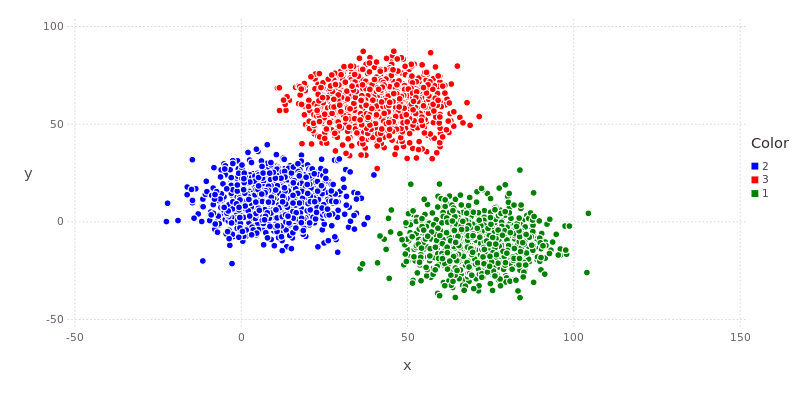
\includegraphics[scale=.25]{clustering}
        \end{figure}
    \end{frame}

    \begin{frame}{Clustering: similarité entre individus}
        \begin{itemize}
            \item La notion de \textbf{similarité} est souvent confondue avec la 
                notion de \textbf{distance}.
            \item La similarité doit être \textbf{adaptée à la nature des 
                données}.
        \end{itemize}

        \begin{table}[!h]
            \centering
               \begin{tabular}{cc}
               \hline
               Euclidienne & $ ||a - b ||_2  = \sqrt{ \sum_{i} (a_i - b_i)^2} $    \\	
               \hline
               Manhattan & $ ||a - b ||_1  = \sum_{i} |a_i - b_i|$    \\	
               \hline
               Maximum & $ ||a - b ||_{\infty}  = \mathop\mathrm{max}_{i} |a_i - b_i|$    \\	
               \hline 
               Mahalanobis & $ \sqrt{(a-b)^\top S^{-1}(a-b)}$    \\	
               \hline  
               Hamming & $ Hamming(a,b) = \sum_i  (1- \delta_{a_i,b_i}) $   \\	
               \hline           
               \end{tabular}
               \caption{Exemples de distances}
           \end{table}
    \end{frame}

    \begin{frame}{Clustering: types de partitions}
        Après un clustering, on obtient une partition de l'espace ainsi que les 
        appartenances des individus à chaque groupe de cette partition. Ces 
        appartenances peuvent être \textbf{dures}, \textbf{molles} ou 
        \textbf{floues}.

        \begin{table}[htbp]
            \centering
            \begin{subtable}{.3\textwidth}
                \centering
                \begin{tabular}{|c|c|c|c|}
                    \hline
                          & $c_1$       & $c_2$ & $c_3$ \\
                    \hline
                    \hline
                    $x_1$   & 1    &  0       &  0 \\
                    $x_2$   & 0    &  1       &  0 \\
                    $x_3$   & 0    &  0       &  1 \\
                    $x_4$   & 0    &  0       &  1 \\
                    \hline  
                \end{tabular}
                \caption{Clustering dur}
            \end{subtable}
            \begin{subtable}{.3\textwidth}
                \centering
                \begin{tabular}{|c|c|c|c|}
                    \hline
                          & $c_1$       & $c_2$ & $c_3$ \\
                    \hline
                    \hline
                    $x_1$   & 1    &  1       &  0 \\
                    $x_2$   & 0    &  1       &  1 \\
                    $x_3$   & 0    &  0       &  1 \\
                    $x_4$   & 0    &  0       &  1 \\
                    \hline
                \end{tabular}
                \caption{Clustering mou}
            \end{subtable}
            \begin{subtable}{.3\textwidth}
                \centering
                \begin{tabular}{|c|c|c|c|}
                    \hline
                          & $c_1$       & $c_2$ & $c_3$ \\
                    \hline
                    \hline
                    $x_1$   & 0.9    &  0.1       &  0 \\
                    $x_2$   & 0    &  0.8       &  0.2 \\
                    $x_3$   & 0    &  0.3       &  0.7 \\
                    $x_4$   & 0    &  0       &  1.0 \\
                    \hline
                \end{tabular}
                \caption{Clustering flou}
            \end{subtable}
            \caption{Les trois principaux types d'appartenances à des clusters}
        \end{table}
    \end{frame}

    \begin{frame}{Clustering: différentes approches}
        On peut regrouper les algorithmes de clustering en sous-catégories 
        suivant l'approche qu'ils utilisent:
        \begin{itemize}
            \item \textbf{Méthodes hiérarchiques}: création d'un arbre de 
                correspondance entre les individus (Agglomerative method).
            \item \textbf{Méthodes de quantification de vecteurs}: définition 
                d'individus prototypes pour synthétiser les individus en entrée 
                (K-Means).
            \item \textbf{Méthodes de densité}: estimation des clusters suivant 
                les zones les plus densément peuplées de l'espace d'entrée 
                (DBSCAN).
            \item \textbf{Méthodes stochastiques}: création de modèles 
                probabilistes définissant la probabilité d'appartenance d'un 
                individu à un cluster donné (GMM).
        \end{itemize}
    \end{frame}

    \begin{frame}{Clustering: approche multi-vues}
        Apparition d'un nouveau contexte: \textbf{un même ensemble d'individu} 
        est décrit dans plusieurs base de données indépendantes appelées 
        \textbf{vues}.

        \textbf{Problème}: comment obtenir un clustering de cet ensemble 
        d'individus ?

        Deux approches:
        \begin{itemize}
            \item<2-> {\only<4>{\color{lightgray}}\textbf{Coopérative}: chaque 
                vue effectue un clustering de ses données locales avant de 
            transférer ses résultats à une entité tiers qui devra fusionner les 
        résultats.}
            \item<3-> \textbf{Collaborative}: chaque vue effectue un premier 
                clustering local, puis le modifie en fonction des résultats 
                obtenus par les autres vues.
        \end{itemize}
    \end{frame}

    \begin{frame}{Clustering: approche multi-vues}
        Exemple multi-vues
        \begin{itemize}
            \item \textbf{Vue 1}: Ensemble des achats récent d'un individus 
                sur des sites d'e-commerce
            \item \textbf{Vue 2}: Salaire et régime alimentaire
            \item \textbf{Vue 3}: Contenu des derniers repas de chaque 
                individu
        \end{itemize}
    \end{frame}

    \begin{frame}{Clustering collaboratif: définition}
        Le \textbf{clustering collaboratif} est un domaine récent désignant 
        l'ensemble des méthodes permettant à \textbf{plusieurs algorithmes de 
        clustering} opérant sur des \textbf{sources de données différentes} de 
        collaborer pour \textbf{améliorer localement} leurs résultats.

        \begin{itemize}
            \item Les algorithmes utilisés peuvent être \textbf{différents}.
            \item Les vues doivent partager soit leurs descripteurs (clustering 
                vertical), soit \textbf{leurs individus} (clustering horizontal) 
                pour pouvoir être comparées.
        \end{itemize}
        \begin{figure}[b]
            \centering
            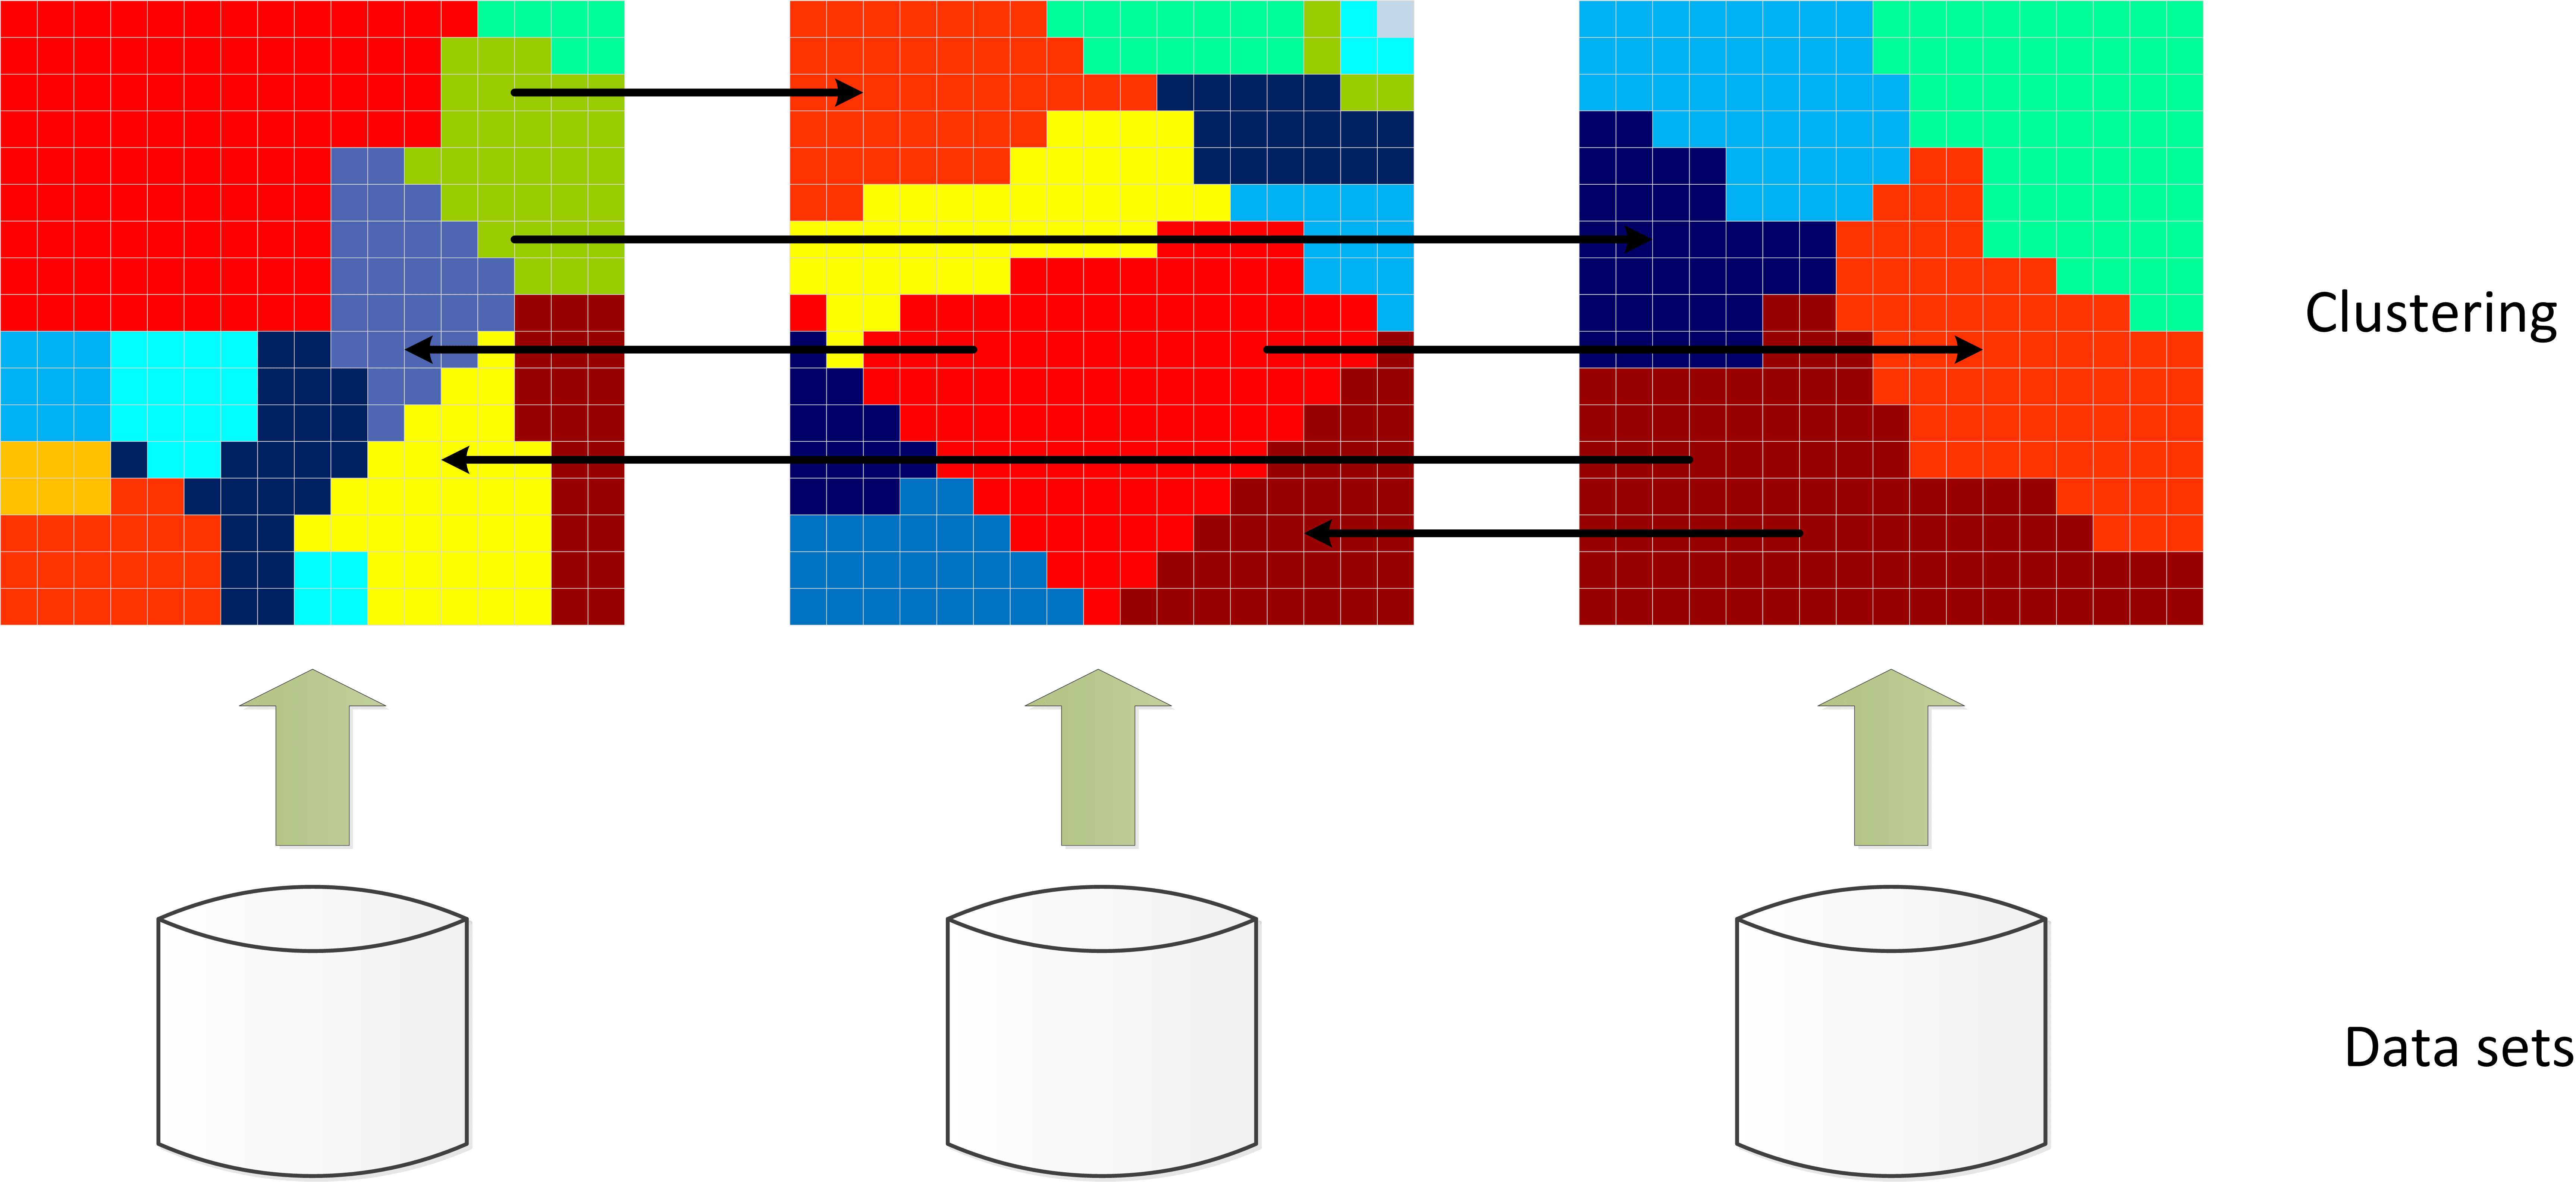
\includegraphics[scale=0.02]{hcc-min}
            \caption{Illustration du principe de clustering collaboratif 
            horizontal}
        \end{figure}
    \end{frame}

    \begin{frame}{Clustering collaboratif: processus}
        \begin{figure}[b]
            \centering
            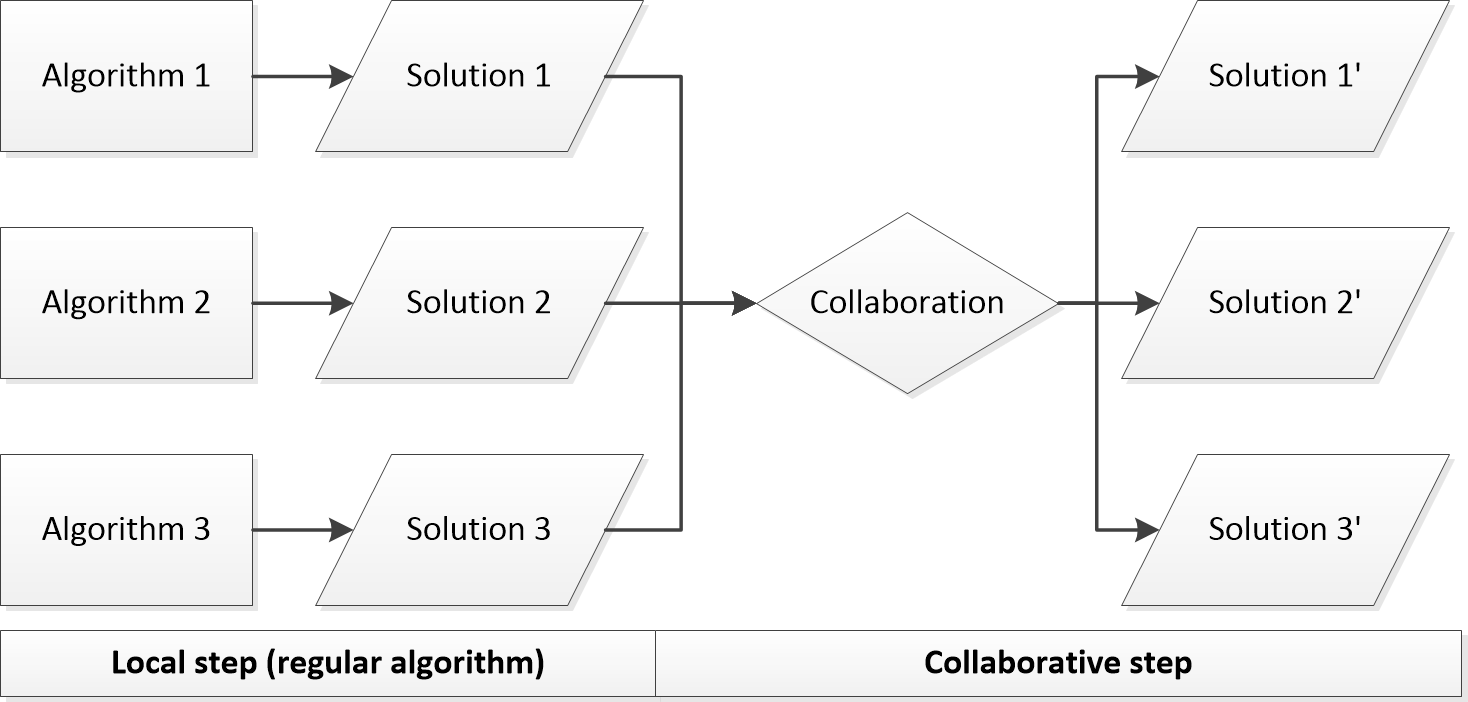
\includegraphics[scale=.70]{clusteringcoll}
            \caption{Processus de clustering collaboratif}
        \end{figure}
    \end{frame}

    %\begin{frame}{Clustering collaboratif: théorie}
        %Définition d'un critère $Q^i$ à optimiser pour chaque vue $V_i$:
        %\begin{align*}
            %$Q^i &= \alpha_i Q^i_{local}(V_i) + Q^i_{collab}(V_i, V_{j\neq i})\\
            %&= \alpha_i Q^i_{local}(V_i) + \sum_{j\neq i} \beta^i_j C_j^i(V_i, V_j)$
        %\end{align*}
        %Avec:
        %\begin{itemize}
            %\item $\alpha_i$ et $\beta_j^i$ les coeffcients de pondération.
            %\item $Q^i_{local}$ et $Q^i_{collab}$ respectivement les 
                %contributions de la vue locale et des vues externes.
            %\item $C_j^i$ la contribution de la vue externe $V_j$, détermine le 
                %degrès de similarité entre $V_i$ et $V_j$.
        %\end{itemize}
    %\end{frame}

    \begin{frame}{Clustering collaboratif: théorie}
        Définition d'un algorithme de clustering collaboratif:
        \begin{itemize}
            \item $Q^i_{local}$ est généralement basé sur \textbf{le critère de 
                l'algorithme local} à optimiser.
            \item $Q^i_{collab}$ se base sur \textbf{l'échange d'information 
                entre vues}, typiquement les appartenances des individus aux 
                clusters respectifs de chaque vue.
            \item $\alpha_i$ et $\beta_j^i$ sont définis \textbf{à la main}.  
                L'approximation $\forall j, \beta_j^i = \alpha_i^2$ est parfois 
                utilisée car donnant de bons résultats en pratique.
        \end{itemize}
    \end{frame}

    \section{Clustering collaboratif incrémental}
        \begin{frame}{Contexte}
            \textit{Objectif du clustering collaboratif}: définir un ensemble de 
            clusters suivant \textbf{la distribution} des données fournies en 
            entrée.

            \textbf{Problème}: il arrive que cette distribution \textbf{évolue 
            au cours du temps}

            \textbf{Exemple}: évolution du régime alimentaire d'un individu ou 
            de la répartition des salaires à l'échelle d'une population.

            \begin{figure}[b]
                \centering
                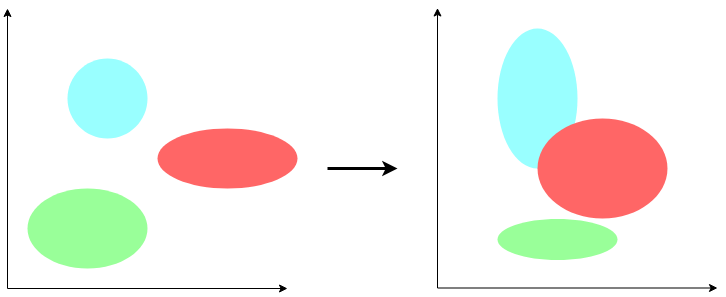
\includegraphics[scale=.2]{changedistrib}
            \end{figure}

            Utilisation du clustering \textbf{incrémental}: les clusters sont 
            appris au cours du temps afin de \textbf{s'adapter} aux éventuels 
            changements de distribution. On utilise les $N_{batch}$ derniers 
            individus comme échantillon d'apprentissage.

        \end{frame}

        \begin{frame}{Clustering collaboratif incrémental}
            Définition d'une méthode de clustering incrémental:
            \begin{itemize}
                \item<2-> Choix de la méthode de clustering
                \item<3-> Adaptation de la méthode de clustering pour de 
                    l'apprentissage incrémental
                \item<4-> Adaptation du clustering collaboratif au modèle de 
                    clustering obtenu
            \end{itemize}
        \end{frame}

        \begin{frame}{Choix de la méthode de clustering}

            Dans notre cas, utilisation des \textbf{cartes auto-adaptatrices de 
            Kohonen} (ou Self-Organizing Maps (SOM) en anglais) comme méthode de 
            clustering.

            \begin{itemize}
                \item \textbf{$\mathbf{1^{ère}}$ contrainte}: des individus 
                    correspondants doivent appartenir à des \textbf{prototypes 
                    correspondants} ou à leurs voisinnages proches.
                \item \textbf{$\mathbf{2^{ème}}$ contrainte}: \textbf{même 
                    topologie des cartes} pour toutes les vues pour les rendre 
                    comparables.
            \end{itemize}

            \begin{figure}[b]
                \centering
                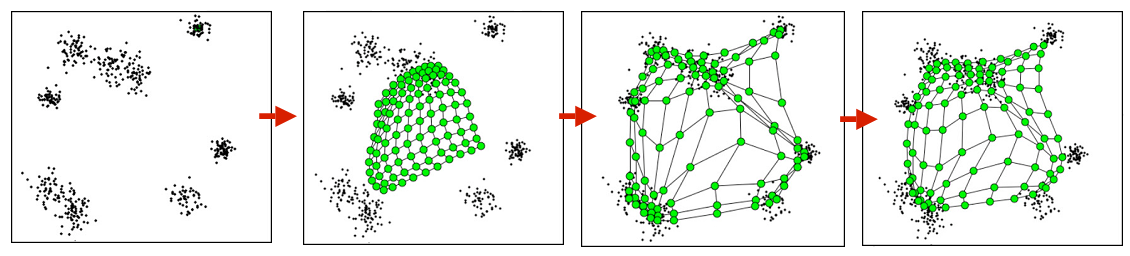
\includegraphics[scale=.43]{SOM2}
                \caption{Exemple de SOM}
            \end{figure}
        \end{frame}

        \begin{frame}{Cartes Auto-Adaptatrices (SOM)}
            \begin{itemize}
                \item Méthode à base de \textbf{prototypes} (quantification de 
                    vecteurs)
                \item Permet la \textbf{visualisation} de données en hautes 
                    dimensions
                \item Notion de \textbf{voisinage}: utilisation d'une 
                    \textbf{fonction de température}.
            \end{itemize}

            \begin{equation*}
                \lambda(t) = 
                \lambda_{min}\left(\frac{\lambda_{max}}{\lambda_{min}}\right)^{\frac{1}{t}}
                \qquad
                K_{i,j} = \exp\left(-\frac{d^2_1(i,j)}{\lambda(t)}\right)
            \end{equation*}

            \begin{figure}[b]
                \centering
                \begin{subfigure}[b]{0.45\textwidth}
                    \centering
                    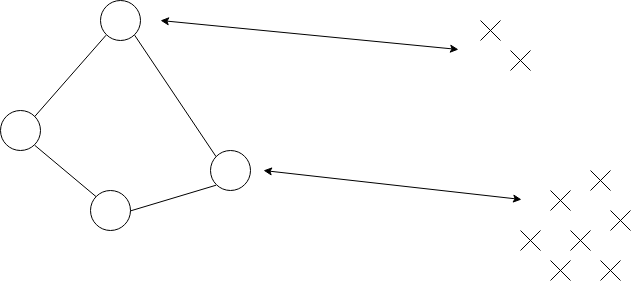
\includegraphics[scale=.2]{somhot}
                    \caption{Température élevée}
                \end{subfigure}
                \begin{subfigure}[b]{0.45\textwidth}
                    \centering
                    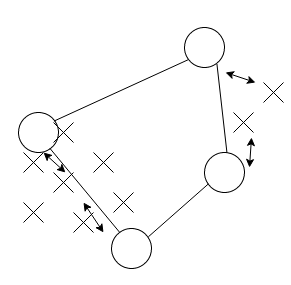
\includegraphics[scale=.25]{somcold}
                    \caption{Température faible}
                \end{subfigure}
            \end{figure}
        \end{frame}

        \begin{frame}{SOM: version incrémentale}
            Les SOM incrémentales ont déjà été étudiées, mais les solutions 
            proposées se basent toutes sur \textbf{l'ajout de prototypes} 
            (\cite{paplinski2012incremental} et \cite{deng2000esom}).\\
            $\rightarrow$ \textbf{Non applicable au clustering collaboratif} du 
            fait de la seconde contrainte: la topologie doit rester la même pour 
            toutes les cartes.

            \textbf{Limitation}: fonction de température dépendante du 
            \textbf{temps}\\
            \textbf{Solution}: rendre la fonction dépendante des 
            \textbf{individus}
            \begin{equation*}
                \lambda(t) = 
                \lambda_{min}\left(\frac{\lambda_{max}}{\lambda_{min}}\right)^{\frac{1}{t}}
                \quad\rightarrow\quad
                \widetilde{\lambda}(B, W) = 
                \frac{1}{N_{batch}}\sum_{i=1}^{N_{batch}}\|x_i - \chi(x_i)\|_2
            \end{equation*}
            \vspace{.1cm}
        \end{frame}

        \begin{frame}{SOM et clustering collaboratif}
            L'application des SOM au clustering collaboratif se fait en 
            définissant les termes précemment définis:

            \begin{equation*}
            {Q}^m_{local} = 
            \alpha_m\sum_{i=1}^{N}\sum_{j=1}^{|W|}{K}^m_{j, 
            \chi(x_i)}\|x_i^m - \omega_j^m\|^2
            \end{equation*}

            \begin{equation*}
            {Q}^m_{collab} = \sum_{m'=1, m'\neq 
            m}^{P}\beta_m^{m'}\sum_{i=1}^{N}\sum_{j=1}^{|W|}({K}^m_{j, 
            \chi(x_i)} - {K}^{m'}_{j, \chi(x_i)})^2  \|x_i^m - \omega_j^m\|^2
            \end{equation*}

            \begin{itemize}
                \item $W$ $\rightarrow$ la carte de prototypes
                \item $\chi(x_i)$ $\rightarrow$ la fonction retournant le 
                    prototype le plus proche de $x_i$.
                \item $x_i^k$ $\rightarrow$ l'individu $i$ dans la vue $m$
                \item $\omega_j^m$ $\rightarrow$ le prototype $j$ de la SOM de 
                    la vue m.
            \end{itemize}
        \end{frame}
    

        \begin{frame}{SOM incrémentale et clustering collaboratif}
            Adaptation de notre version de SOM incrémentale au clustering 
            collaboratif:
            \begin{center}
            $\lambda \rightarrow \widetilde{\lambda}$
            \\~\\
            $K_{i,j}(\lambda) \rightarrow K_{i,j}(\widetilde{\lambda}) 
            \rightarrow \widetilde{K_{i,j}}$
            \\~\\
            $Q_{local}^m / Q_{collab}^m (K_{i,j}) \rightarrow Q_{local}^m / 
            Q_{collab}^m (\widetilde{K_{i,j}}) \rightarrow 
            \widetilde{Q}_{local}^m / \widetilde{Q}_{collab}^m$
            \end{center}
            Le nouveau critère dépendant dépendant uniquement des $N_batch$ 
            derniers individus apparus, il est possible d'effectuer un 
            \textbf{apprentissage collaboratif incrémental} sur l'ensemble des 
            vues.

            Les règles de mise à jour sont obtenus par \textbf{descente de 
            gradient} appliquée sur ce critère.
        \end{frame}

        \begin{frame}{Expérimentations}
            \begin{itemize}
                \item Analyse de l'impact du clustering collaboratif sur
                    l'apprentissage incrémental.
                \item Application directe de la phase collaborative pour le
                    clustering collaboratif pour pouvoir comparer les
                    résultats aux version locales.
                \item Variation de la taille du batch pour étudier l'impact
                    sur l'apprentissage.
            \end{itemize}
        \end{frame}
        
        \begin{frame}{Expérimentations}
            Test de notre méthode sur 4 jeux de données différents
            \begin{itemize}
                \item Spambase
                \item Waveform
                \item Wisconsin Breast Cancer Diagnosis (WDBC)
                \item Isolet
            \end{itemize}

            \textbf{Pureté d'une SOM}: pureté moyenne de ses prototypes.
            \textbf{Pureté d'un prototype}: classe majoritaire parmi les
            individus associés à ce prototype

            \textbf{Erreur moyenne de quantification}: distance moyenne
            entre un prototype et les individus qui y sont associés.

            \begin{equation*}
                qe = \frac{1}{N_{batch}}\sum_{i=1}^{N_{batch}}\|x_i -
                \omega_{\chi(x_i)}\|^2
            \end{equation*}
        \end{frame}

        \begin{frame}{Expérimentations: résultats}
            \begin{table}[!h]
                \caption{Erreur de quantification moyenne pour chaque base
                de donnée. Les nombres en gras sont les plus petits pour
            chaque ligne}
                \begin{center}
                    \resizebox{.6\columnwidth}{!}{
                        \begin{tabular}{cccc}
                                       & Vue & SOM Incrémentales & \begin{tabular}[c]{@{}c@{}}Clustering Collaboratif\\Incrémentale\end{tabular} \\ \midrule
            \multirow{3}{*}{Spam Base} & 1    & 0.31            & \textbf{0.26}                                                                  \\
                                       & 2    & \textbf{0.18}   & 0.19                                                                           \\
                                       & 3    & 0.18            & \textbf{0.16}                                                                  \\ \midrule
            \multirow{3}{*}{Waveform}  & 1    & \textbf{0.18}   & 0.23                                                                           \\
                                       & 2    & \textbf{0.17}   & 0.19                                                                           \\
                                       & 3    & \textbf{0.24}   & 0.30                                                                           \\ \midrule
            \multirow{3}{*}{WDBC}      & 1    & \textbf{0.19}   & 0.19                                                                           \\
                                       & 2    & \textbf{0.16}   & 0.19                                                                           \\
                                       & 3    & 0.20            & \textbf{0.16}                                                                  \\ \midrule
            \multirow{3}{*}{Isolet}    & 1    & 2.15            & \textbf{1.27}                                                                  \\
                                       & 2    & 2.84            & \textbf{1.38}                                                                  \\
                                       & 3    & 2.85            & \textbf{1.37}                                                                 \\ \midrule
                        \end{tabular}
                    }
                \end{center}
            \end{table}
        \end{frame}

        \begin{frame}{Expérimentations: résultats sur Isolet}
            \begin{figure}[!h]
                \centering
                \begin{subfigure}[b]{0.3\textwidth}
                    \centering
                    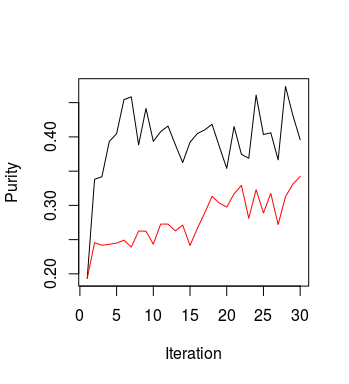
\includegraphics[width=0.7\textwidth, trim= 0cm 0.5cm 1cm 2cm, clip]{img/11.png}
                    \caption{$N_{batch}=10$, View 1}
                \end{subfigure}
                \begin{subfigure}[b]{0.3\textwidth}
                    \centering
                    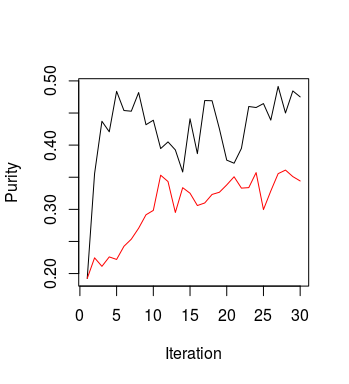
\includegraphics[width=0.7\textwidth, trim= 0cm 0.5cm 1cm 1.73cm, clip]{img/22.png}
                    \caption{$N_{batch}=10$, View 2}
                \end{subfigure}
                \begin{subfigure}[b]{0.3\textwidth}
                    \centering
                    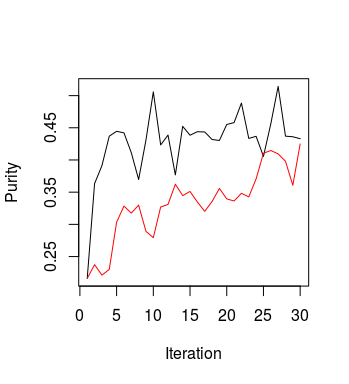
\includegraphics[width=0.7\textwidth, trim= 0cm 0.5cm 1cm 2cm, clip]{img/33.png}
                    \caption{$N_{batch}=10$, View 3}
                \end{subfigure}\\
                \begin{subfigure}[b]{0.3\textwidth}
                    \centering
                    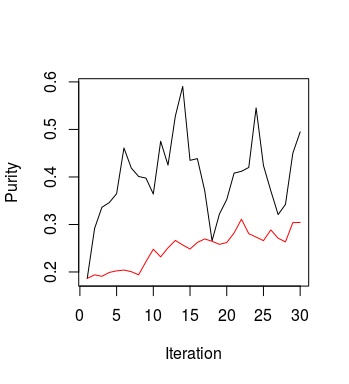
\includegraphics[width=0.7\textwidth, trim= 0cm 0.5cm 1cm 1.9cm, clip]{img/p1.png}
                    \caption{$N_{batch}=3$, View 1}
                \end{subfigure}
                \begin{subfigure}[b]{0.3\textwidth}
                    \centering
                    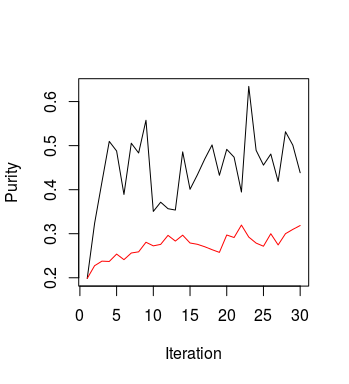
\includegraphics[width=0.7\textwidth, trim= 0cm 0.5cm 1cm 2cm, clip]{img/p2.png}
                    \caption{$N_{batch}=3$, View 2}
                \end{subfigure}
                \begin{subfigure}[b]{0.3\textwidth}
                    \centering
                    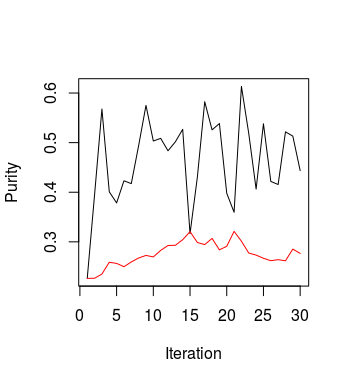
\includegraphics[width=0.7\textwidth, trim= 0cm 0.5cm 1cm 2cm, clip]{img/p3.png}
                    \caption{$N_{batch}=3$, View 3}
                \end{subfigure}
                \caption{Évolution des puretés pour Isolet.  Les lignes rouges représentes les SOM incrémentales tandis que les lignes noires représentent les SOM incrémentales collaboratives.  Chaque itération correspond à l'arrivée d'une nouvelle donnée}
            \end{figure}
        \end{frame}

        \begin{frame}{Expérimentations: résultats}
            \begin{itemize}
                \item \textbf{Score en quantification à long termes 
                    comparables}: le
                    clustering collaboratif n'endommage pas les 
                    résultats
                    locaux.
                \item Le clustering collaboratif permet de 
                    \textbf{limiter l'impact
                    du bruit} dans les vues.
                \item Les SOM incrémentales collaboratives 
                    \textbf{apprennent plus
                    vite que les SOM incrémentales seules}: meilleure
                    exploitation de l'information via le partage.
                \item Les SOM collaboratives sont globalement 
                    \textbf{plus instables} que les SOM incrémentales.
                \item La stabilité de l'apprentissage \textbf{augmente 
                    avec la taille du batch}: plus d'informations à 
                    exploiter.
            \end{itemize}
        \end{frame}

    \section{Optimisation de paramètres pour le clustering collaboratif}

    \begin{frame}{Optimisation de paramètres pour le clustering collaboratif}
        \textbf{Objectif}: Apprendre automatiquement les $\alpha$ et les
        $\beta$ en s'affranchissant de simplifications telles que $\beta =
        \alpha^2$.

        Rappel du critère du clustering collaboratif:
        \begin{align*}
            Q^i &= \alpha_i Q^i_{local}(V_i) + Q^i_{collab}(V_i, 
            V_{j\neq i})\\
            &= \alpha_i Q^i_{local}(V_i) + \sum_{j\neq i} \beta^i_j 
            C_j^i(V_i, V_j)
        \end{align*}
        Nous avons proposé une nouvelle méthode de pondération permettant
        d'apprendre automatiquement les poids fixant les importances
        relatives des différents scores.\\
    \end{frame}

    \begin{frame}{Optimisation de paramètres: définition du problème}
        La définition des $\alpha$ et des $\beta$ passe par la résolution
        d'un problème sous contrainte. Les contraintes sont les suivantes :

        \begin{itemize}
            \item<2-> $\beta^* =  
                \operatornamewithlimits{argmin}_{\beta}  \sum_{i \neq j}
        \beta_{i,j}  C _{i,j} $
            \item<3-> $\forall j \quad \prod_{i \neq j}^J \beta_{i,j} = 
                1$
            \item<4-> $\forall (i,j) \quad \beta_{i,j} >0$
            \item<5->{Affranchissement des $\alpha$: comme il s'agit de 
                pondérations relatives, on peut fixer $\alpha=1$.}
        \end{itemize}

        \onslide<6->{\textbf{Objectif:} mettre des poids plus élevés sur 
            les meilleurs accords, tout en gardant une certaine partie 
            des vues en désaccord pour faire évoluer l'information
        }
    \end{frame}

    \begin{frame}{Optimisation de paramètres: méthode de Karush-Kuhn-Tucker}
        Critère + contrainte d'égalité + contrainte d'inégalité\\
        $\rightarrow$ \textbf{méthode de Karush-Kuhn-Tucker (KKT)} 

        \begin{equation*}
        L(\beta,\nu,\lambda)=\sum_{j=1}^J  \sum_{i \neq j}^J ( \beta_{i,j}  C_{i,j}
        - \nu_j  \ln  \beta_{i,j}  - \lambda_{i,j}   \beta_{i,j} ).
        \end{equation*}

        \begin{equation*}
            \frac{\partial L}{\partial \beta_{i,j}} = 0,
            \quad
            \frac{\partial L}{\partial \nu} = 0,
            \quad
            \frac{\partial L}{\partial \lambda} = 0
        \end{equation*}
    \end{frame}
    
    \begin{frame}{Optimisation de paramètres: résultats}
        Après résolution, on obtient:

        \vspace{0.6cm}

        \begin{equation*}
            \forall (i,j), \quad i\neq j \qquad \beta_{i,j} =  
            \frac{(\prod_{k\neq j} C _{k,j})^{\frac 
            1 {J-1}}}{C_{i,j}}
        \end{equation*} 

        \vspace{1cm}
        L'importance d'une vue externe relativement à une vue locale est
        proportionnelle au rapport entre la moyenne géométrique de toutes les
        dissimilarités par rapport à la dissimilarité entre les deux vues
        .\\
        \onslide<2->{$\rightarrow$ \textbf{plus 2 vues sont similaires, 
            plus elles collaboreront.}
        }
    \end{frame}

    \begin{frame}
        \begin{algorithm}[H]
            \caption{Algorithme topologique de collaboration horizontale}
            \textbf{Initialisation:} Initialiser toutes les cartes de
            prototypes $W$ aléatoirement. \\
            \textbf{Étape locale:} Initialisation des cartes\\
            \ForAll{Vue} {
                Minimiser la fonction objectif des cartes auto-adaptatrices
                standards.
            } 
            \textbf{Étape collaborative:}\\
            \ForAll{Vue} {
                Pour $w$ fixé, mettre à jour $\beta$\\
                $ \beta^{*} =  argmin_{\beta}Q(w,\alpha,\beta) $\\
                Pour $\beta$ fixés, mettre à jour les prototypes de 
                toutes les cartes:\\
                $ w^{*} =  argmin_{w}Q(w,\alpha,\beta) $
            }	 
        \end{algorithm}
    \end{frame}

    \begin{frame}{Expérimentations}
        Deux axes d'analyse:
        \begin{itemize}
            \item Analyse de \textbf{l'évolution du critère 
                collaboratif} avec et sans apprentissage automatique des 
                poids.
            \item Analyse des \textbf{valeurs prises par les} $\beta$ en 
                fin d'apprentissage.
        \end{itemize}

        \onslide<2->{Ce que l'on s'attend à trouver:
            \begin{itemize}
                \item Une \textbf{amélioration de la valeur du critère 
                    collaboratif} grâce à notre méthode
                \item \textbf{L'identification automatique des vues 
                    bruitées}, menant à des valeurs de $\beta$ proches de 0.
            \end{itemize}
        }

        \onslide<3->{À noter: pour chaque base de données, \textbf{une 
            vue entièrement composée de bruit} a été rajoutée pour 
            tester le second point.
        }
    \end{frame}

    \begin{frame}{Expérimentations: évolution du critère}
        \begin{figure}[!h]
            \centering
            %\begin{subfigure}[b]{0.3\textwidth}
                %\centering
                %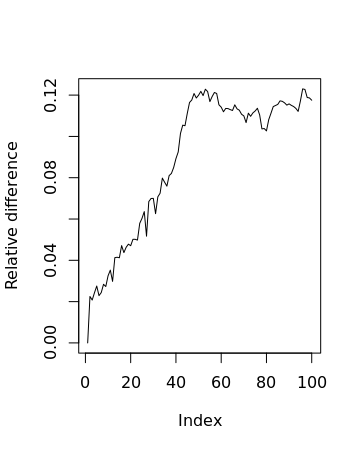
\includegraphics[width=0.8\textwidth]{wdbc_RD.png}
                %\caption{WDBC}
            %\end{subfigure}
            %\begin{subfigure}[b]{0.32\textwidth}
                %\centering
                %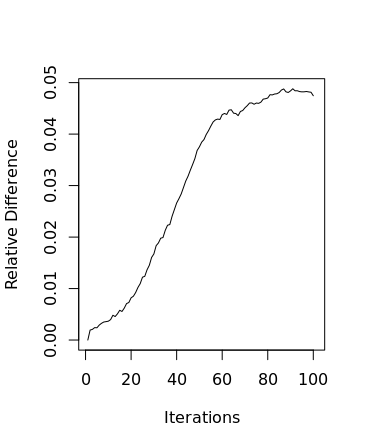
\includegraphics[width=1.0\textwidth]{waveform_RD2.png}
                %\caption{Waveform}
            %\end{subfigure}
            \begin{subfigure}[b]{0.32\textwidth}
                \centering
                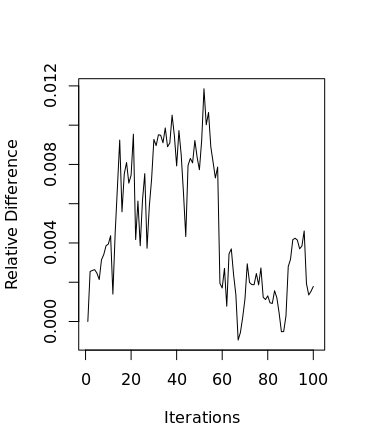
\includegraphics[width=1.0\textwidth]{spambase_RD3.png}
                \caption{Spambase}
            \end{subfigure}
            \begin{subfigure}[b]{0.32\textwidth}
                \centering
                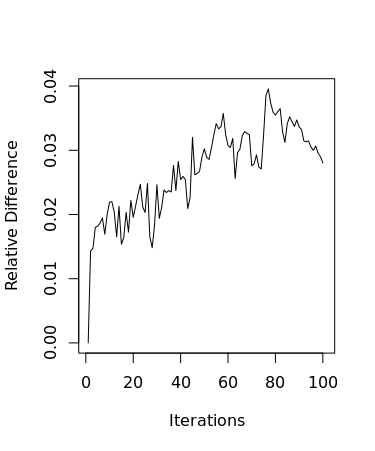
\includegraphics[width=1.0\textwidth]{isolet_RD2}
                \caption{Isolet}
            \end{subfigure}
            \begin{subfigure}[b]{0.32\textwidth}
                \centering
                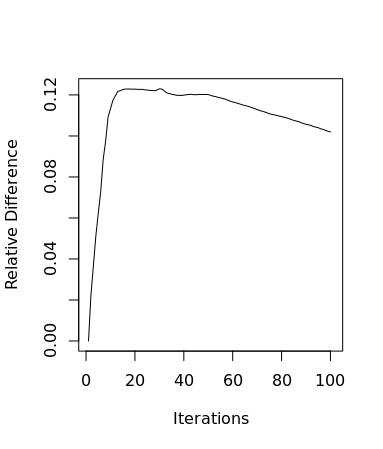
\includegraphics[width=1.0\textwidth]{vhr_RD}
                \caption{VHR Strasbourg}
            \end{subfigure}
            \caption{Relative differences of the weighted criterion with 
                and without $\beta$ optimization all along the learning 
                process
            }
        \end{figure}
    \end{frame}

    \begin{frame}{Expérimentations: évolution du critère}
        \begin{itemize}
            \item \textbf{Amélioration du critère} de manière 
                significative dans la majorité des cas\\~\\
            \item Tous les jeux de données \textbf{ne sont pas traités 
                de la même manière}.
                \begin{itemize}
                    \item Hypothèse: La quantité d'information à 
                        partagée n'est pas toujours la même suivant les 
                        bases considérées.
                \end{itemize}
        \end{itemize}

        Si le critère a été améliorée, c'est peut être parce qu'entre 
        autre, les vues bruitées ont été identifiées ?
    \end{frame}

    \begin{frame}{Expérimentations: identifications des vues bruitées}
        \begin{subfigure}[b]{0.32\textwidth}
            \centering
            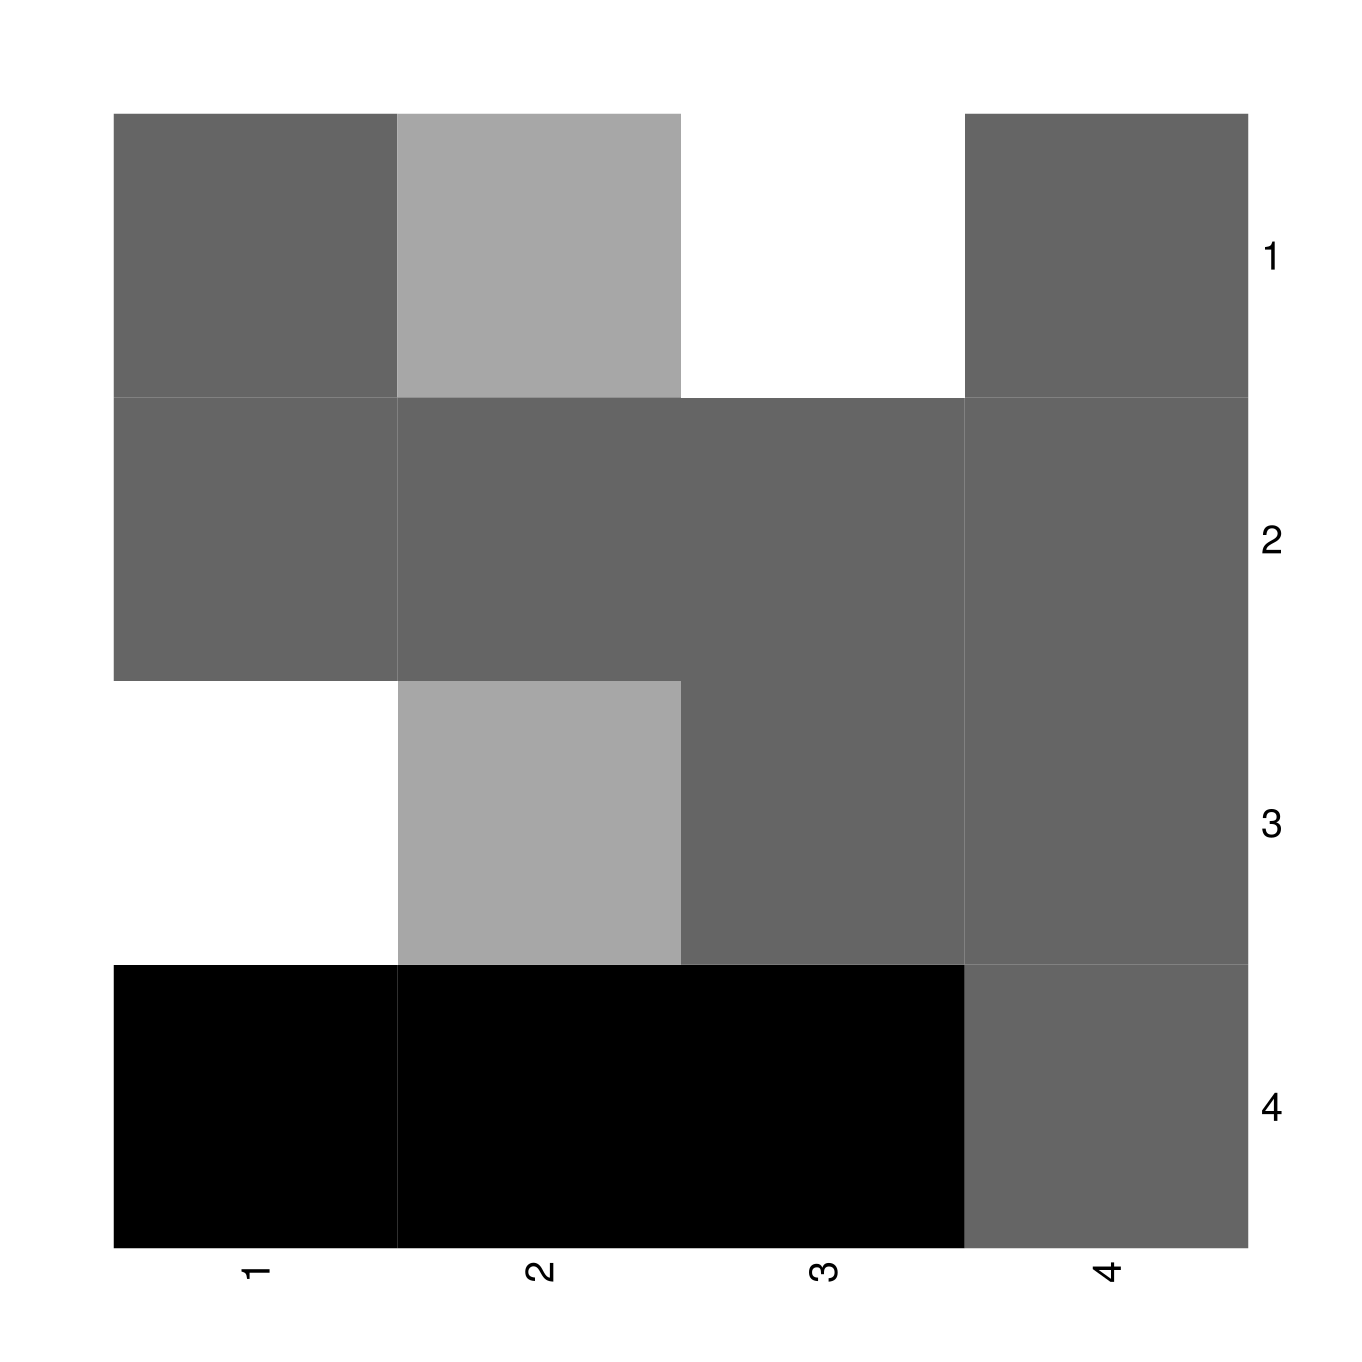
\includegraphics[width=0.33\textwidth]{wdbc_bw}
            \caption{WDBC}
        \end{subfigure}
        \begin{subfigure}[b]{0.32\textwidth}
            \centering
            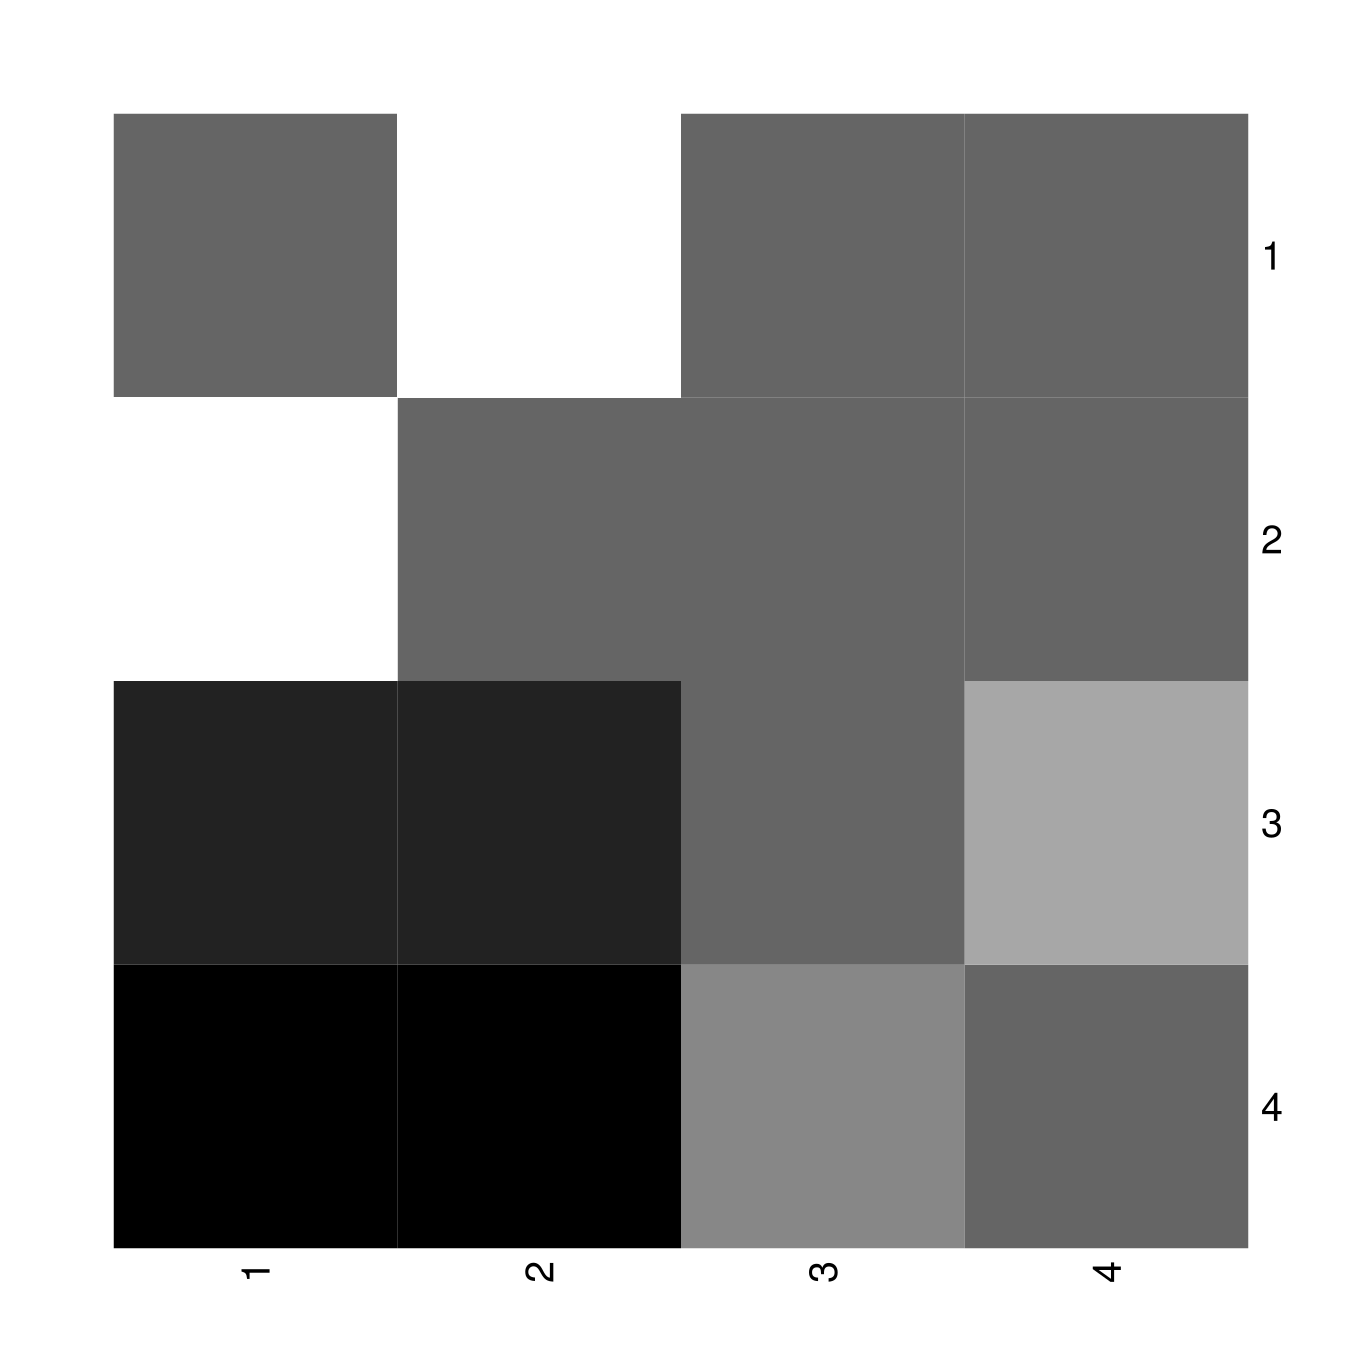
\includegraphics[width=0.33\textwidth]{waveform_bw}
            \caption{Waveform}
        \end{subfigure}
        \begin{subfigure}[b]{0.32\textwidth}
            \centering
            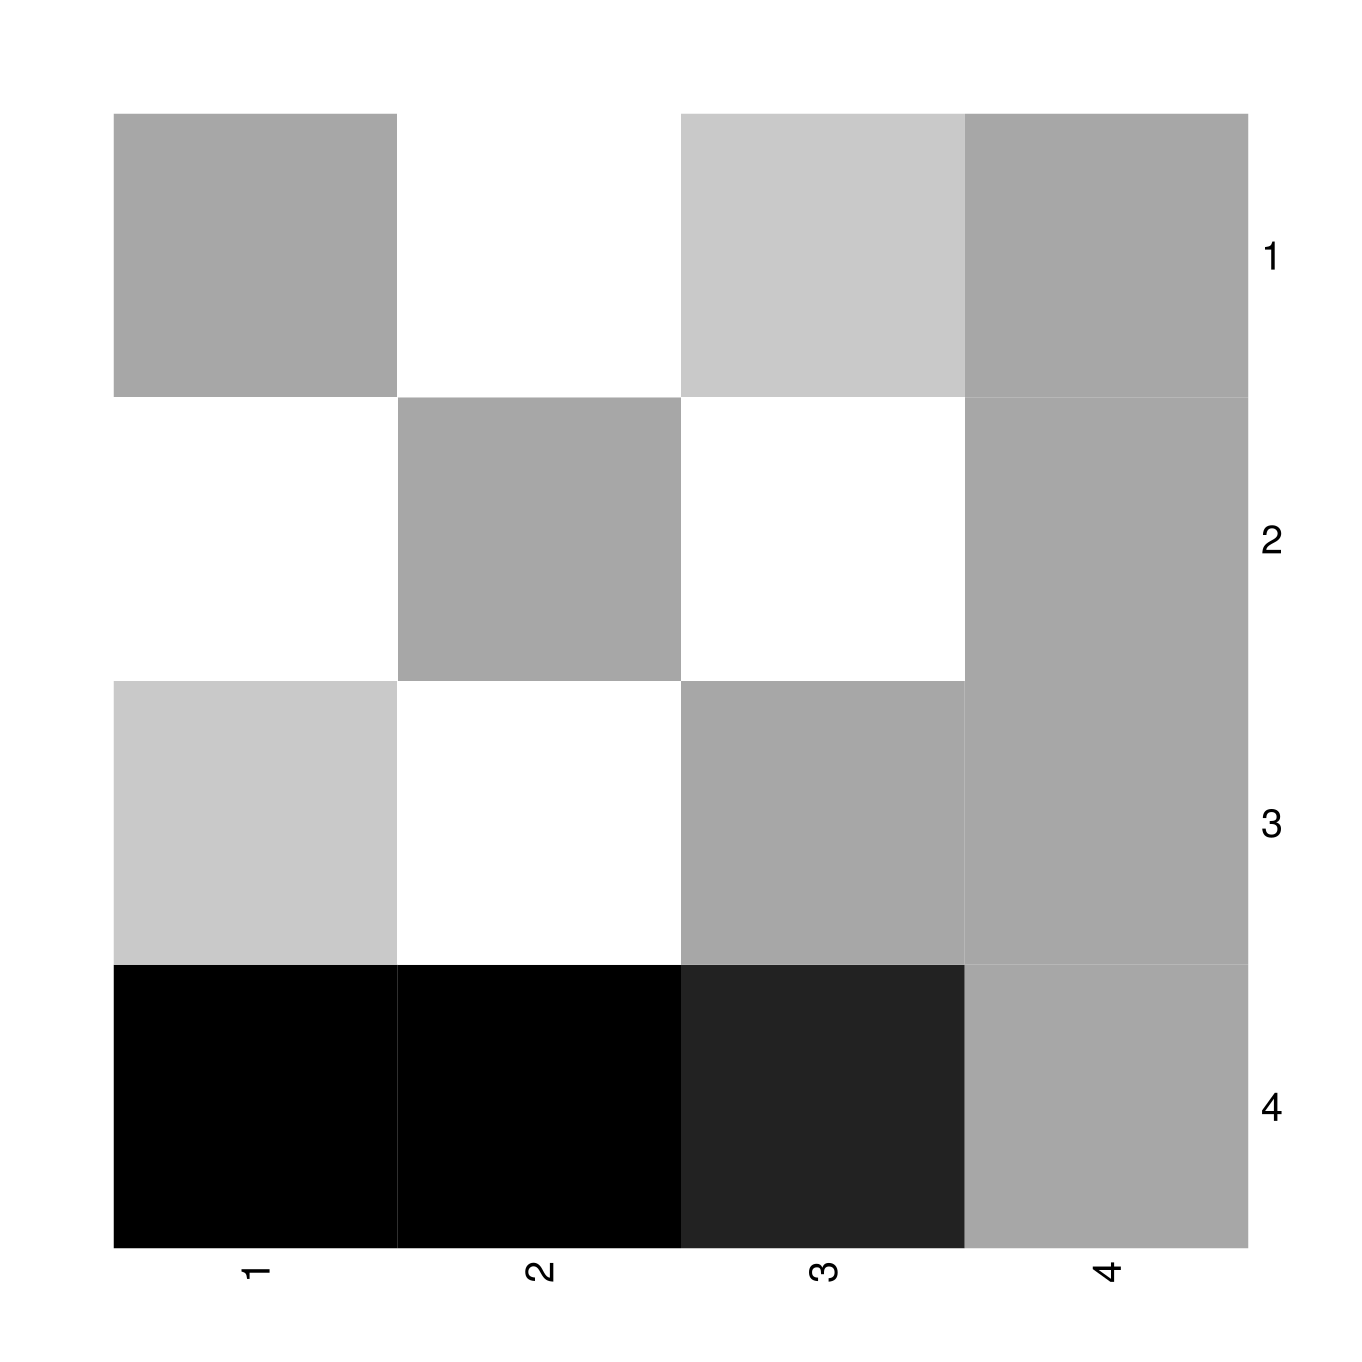
\includegraphics[width=0.33\textwidth]{isolet_bw}
            \caption{Isolet}
        \end{subfigure}
        \caption{Heatmap of the $\beta$ matrices for each dataset.  
            Colors go from white (strong collaboration) to black (weak 
            collaboration). The gray color on the diagonal stands for 
            $\beta=1$.
        }
        \end{figure}
    \end{frame}

    \section{Système de reconstruction collaboratif}
    \begin{frame}
        
    \end{frame}

    \section{Perspectives}
    \begin{frame}
        
    \end{frame}

    \section{Conclusion}
    \begin{frame}
        
    \end{frame}

    \begin{frame}{Bibliographie}
        \bibliographystyle{abbrvnat}
        \bibliography{./bib}
    \end{frame}

\end{document}
